%!TEX root=../../main.tex

\subsection{Breadth-first search}
\subsubsection{Single-Node}
TODO // Hier fehlt noch Giraph, daher noch keine vollständige Auswertung.


In these figures, Galois with 96 threads is shown. Again, we show the impact of Galois' thread count in \autoref{sec:galois_speedup}.
\begin{figure*}
	\begin{subfigure}{0.3\textwidth}
		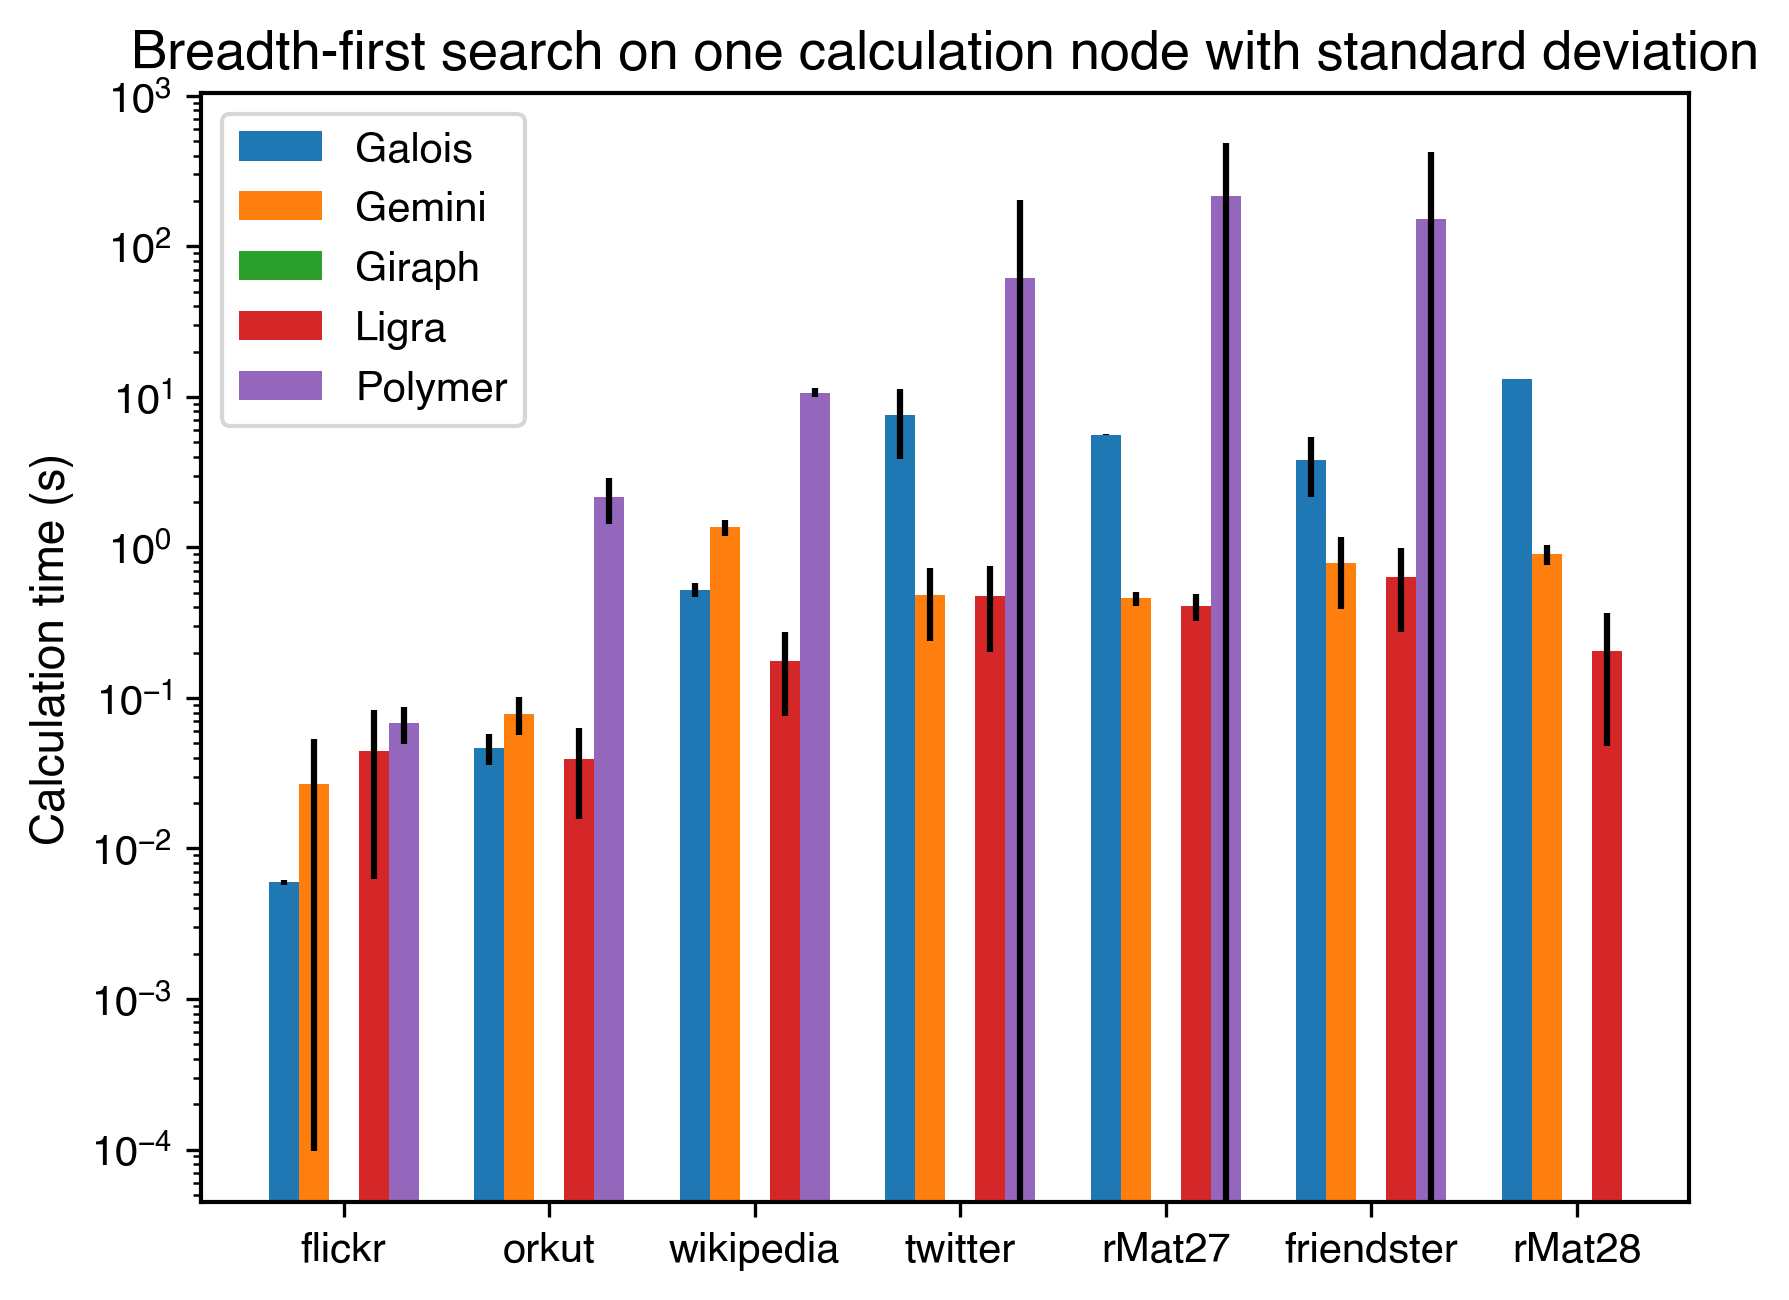
\includegraphics[width=\linewidth]{../../plots/singleNodeBFS_calcTime.png}
		\caption{Calculation times for BFS on a single node}
		\label{fig:singleNodeBFS_calc}
	\end{subfigure}
	\hfil
	\begin{subfigure}{0.3\textwidth}
		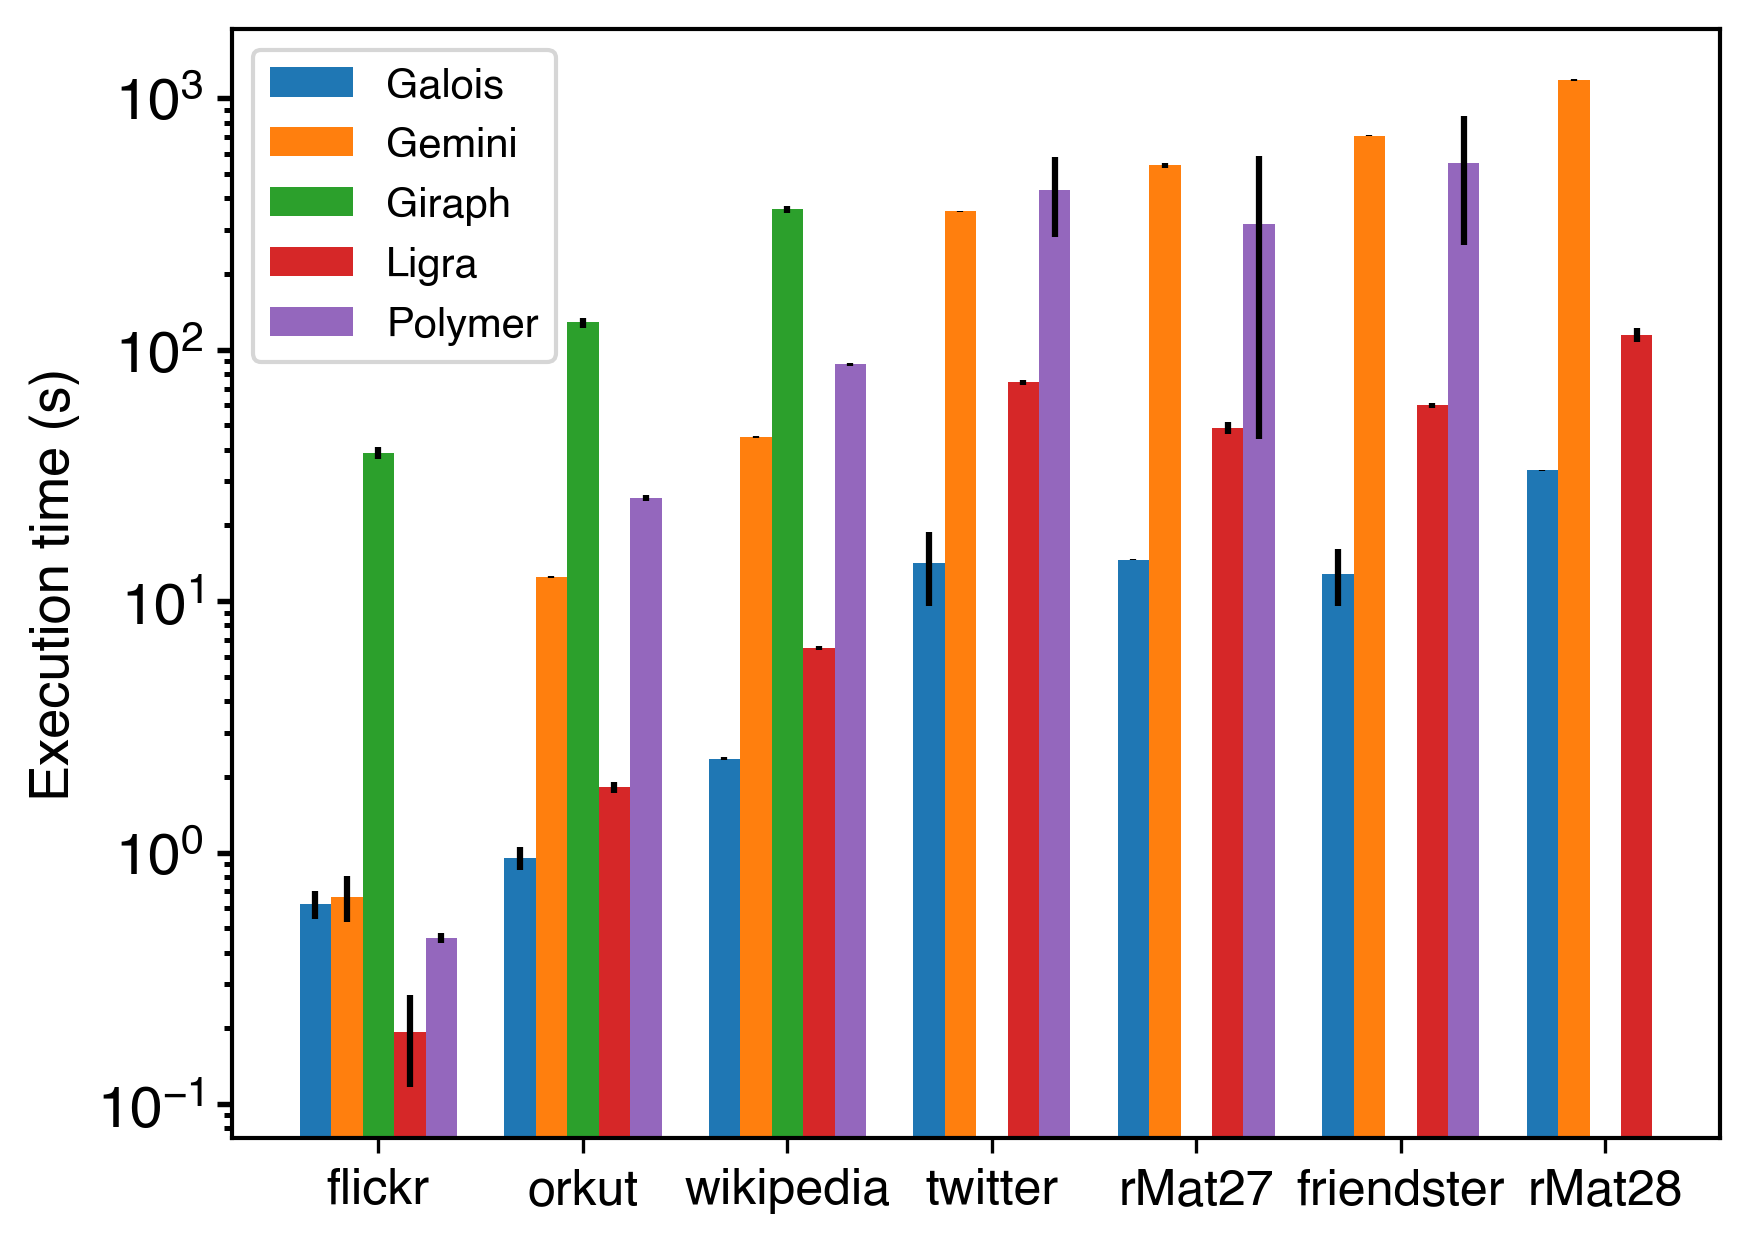
\includegraphics[width=\linewidth]{../../plots/singleNodeBFS_execTime.png}
		\caption{Execution times for BFS on a single node}
		\label{fig:singleNodeBFS_exec}
	\end{subfigure}
	\hfil
	\begin{subfigure}{0.3\textwidth}
		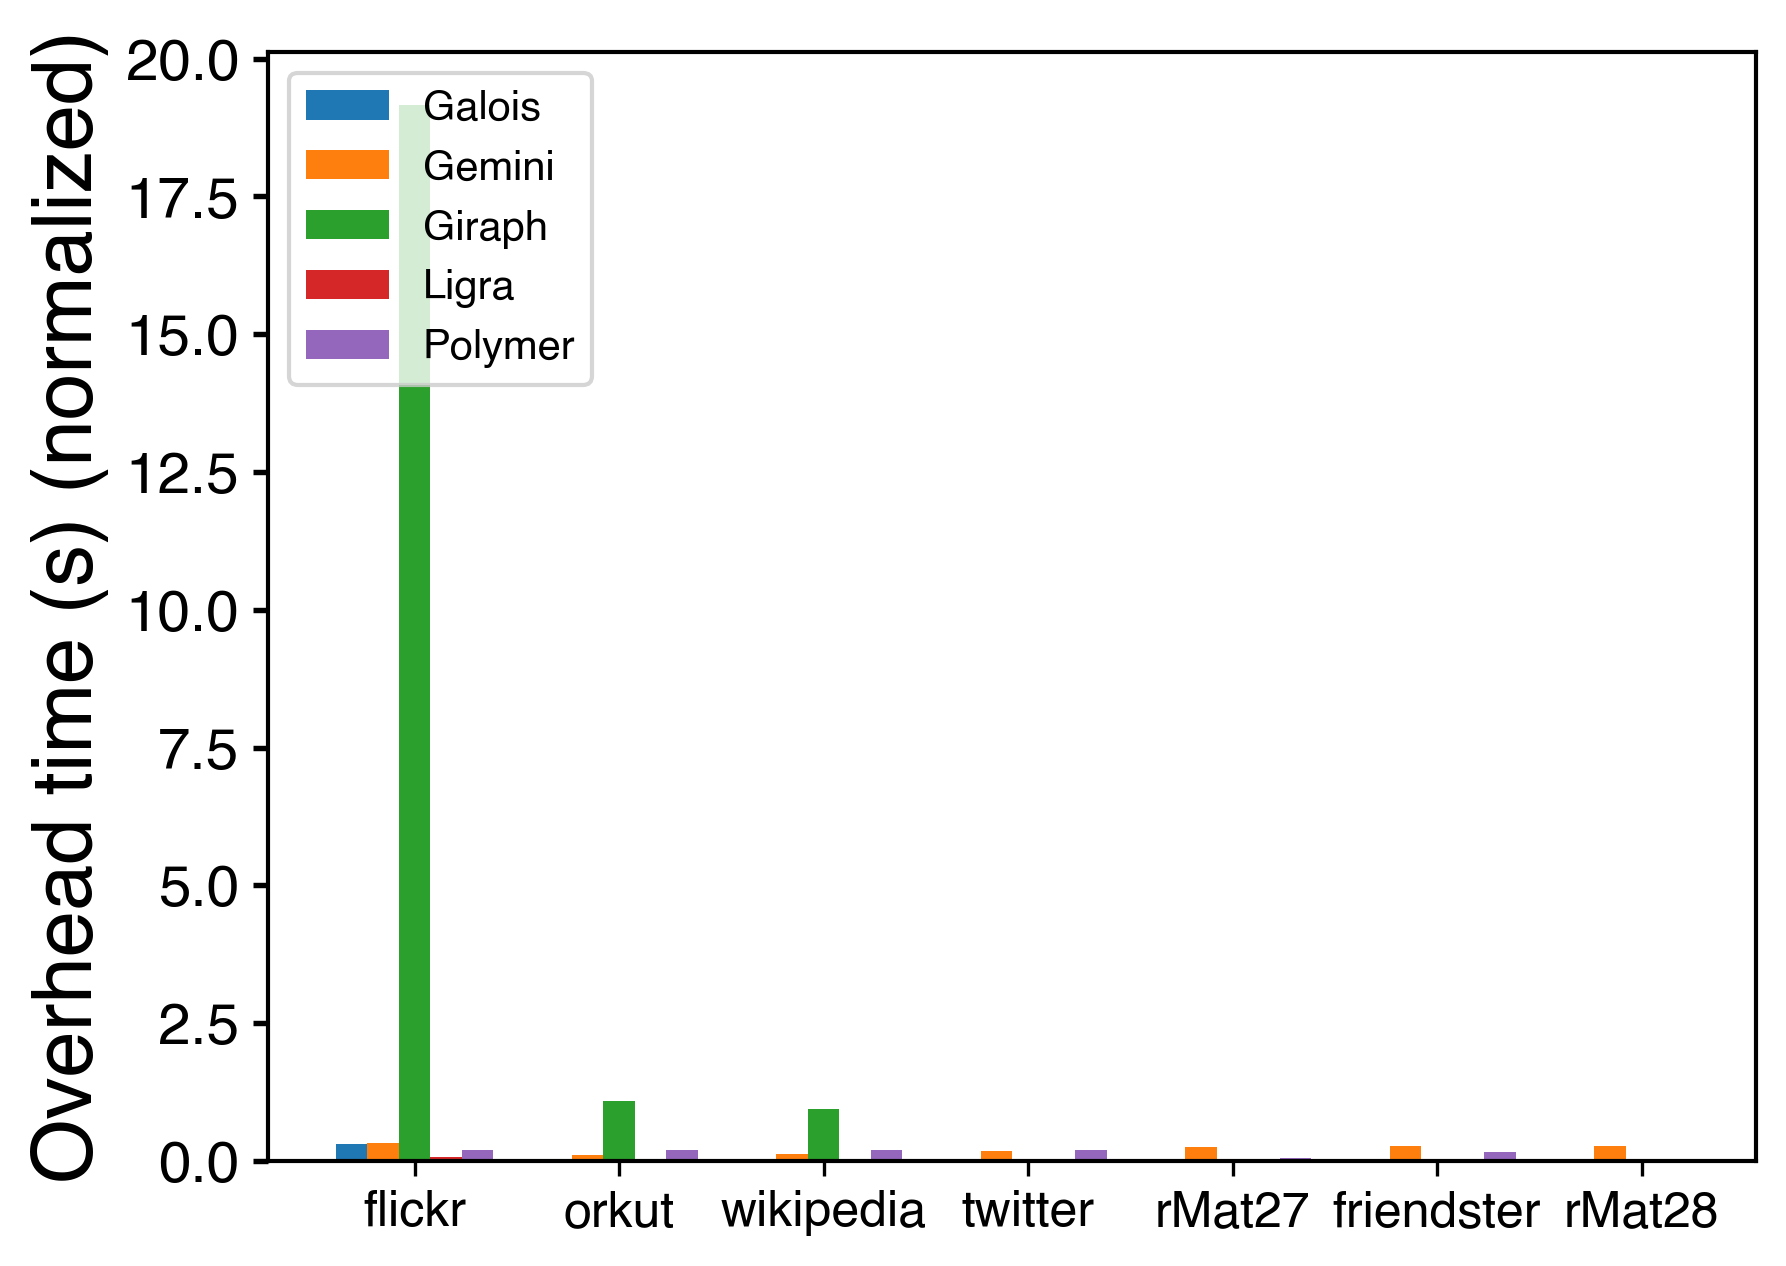
\includegraphics[width=\linewidth]{../../plots/singleNodeBFS_overheadTimeNormalized.png}
		\caption{Overhead time normalized by the graph size in million edges}
		\label{fig:singleNodeBFS_overheadNormalized}
	\end{subfigure}
	
	\caption{Average times on a single computation node, black bars represent one standard deviation in our testing}
\end{figure*}



\subsubsection{Distributed}
\begin{figure}
	\begin{subfigure}{\columnwidth}
		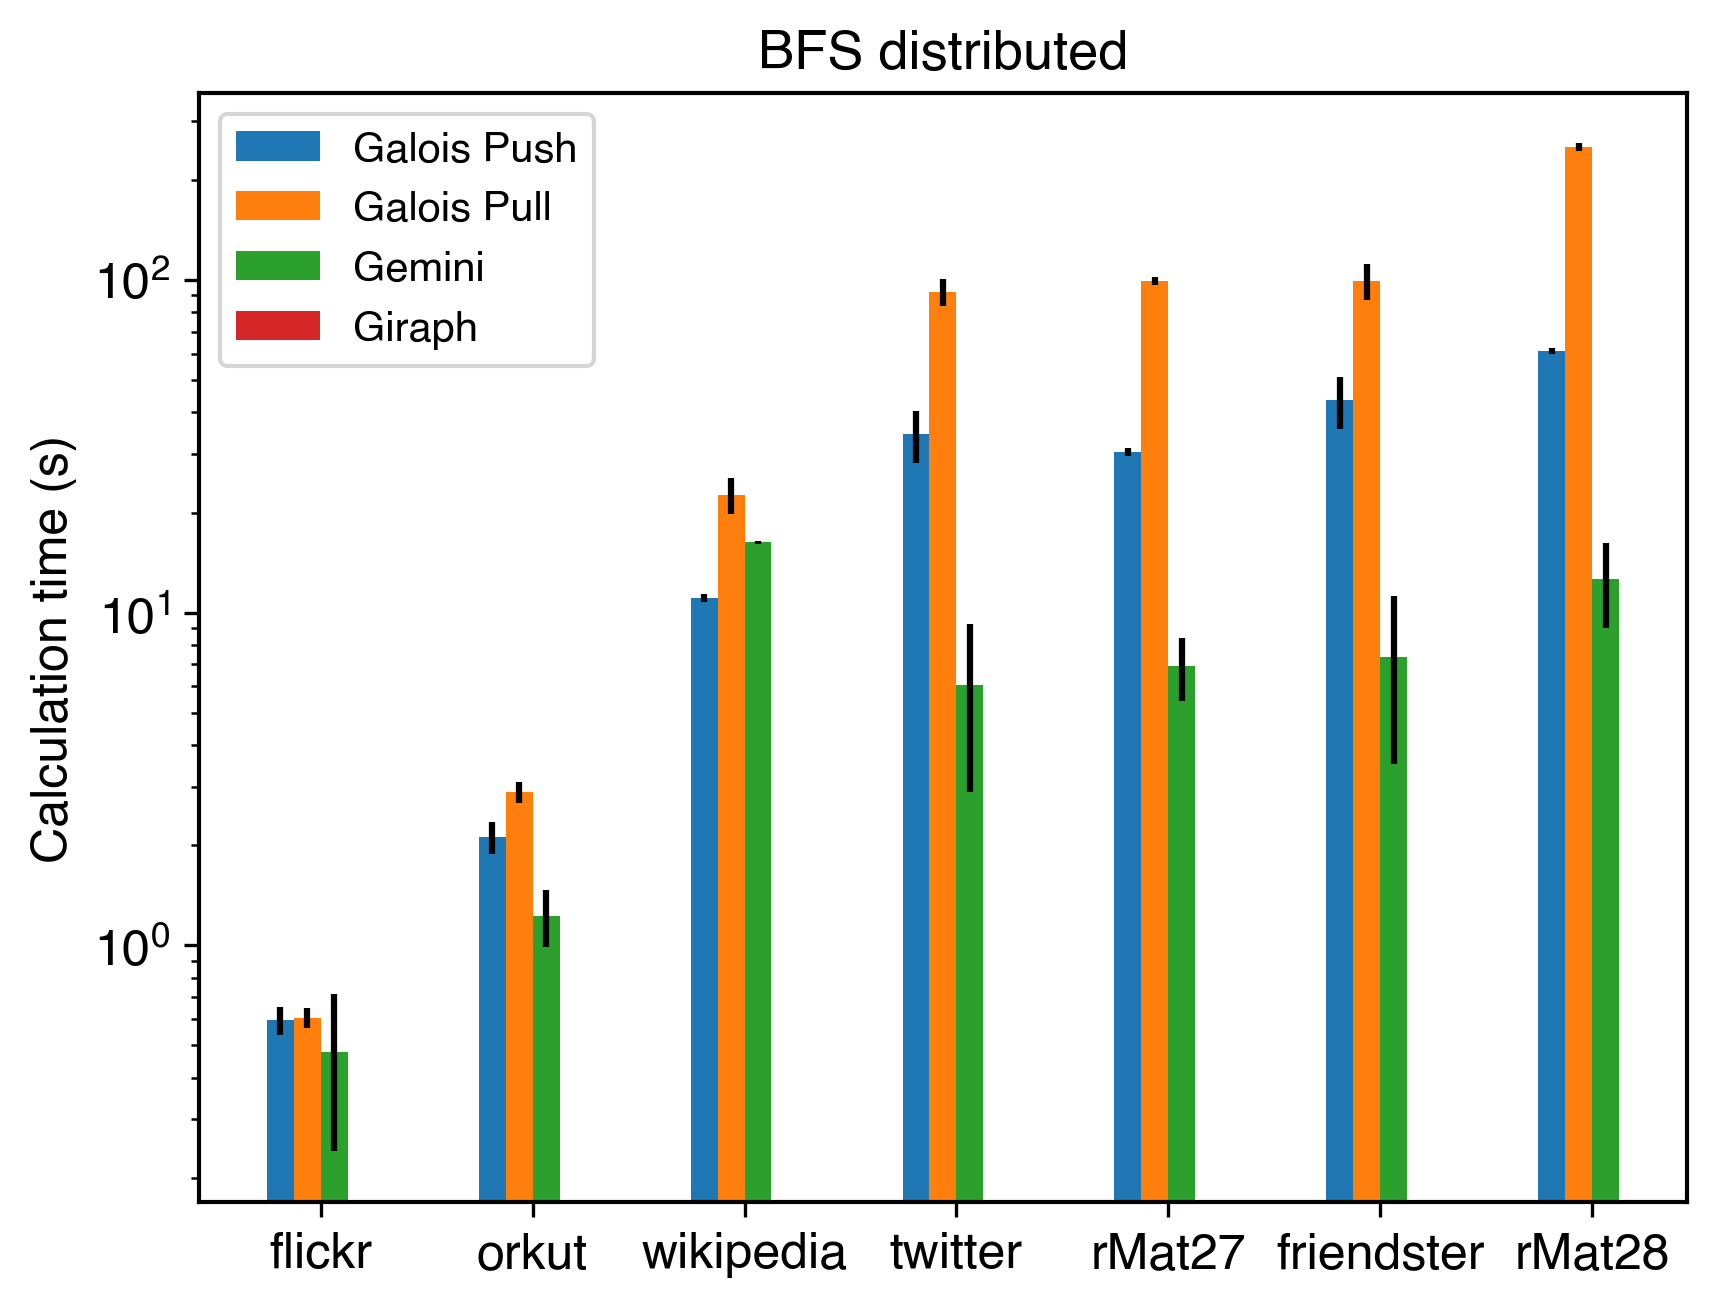
\includegraphics[width=\linewidth]{../../plots/distributedBFS_calcTime.png}
		\caption{Calculation times for distributed BFS}
		\label{fig:distributedBFS_calc}
	\end{subfigure}
	% \hfil
	\begin{subfigure}{\columnwidth}
		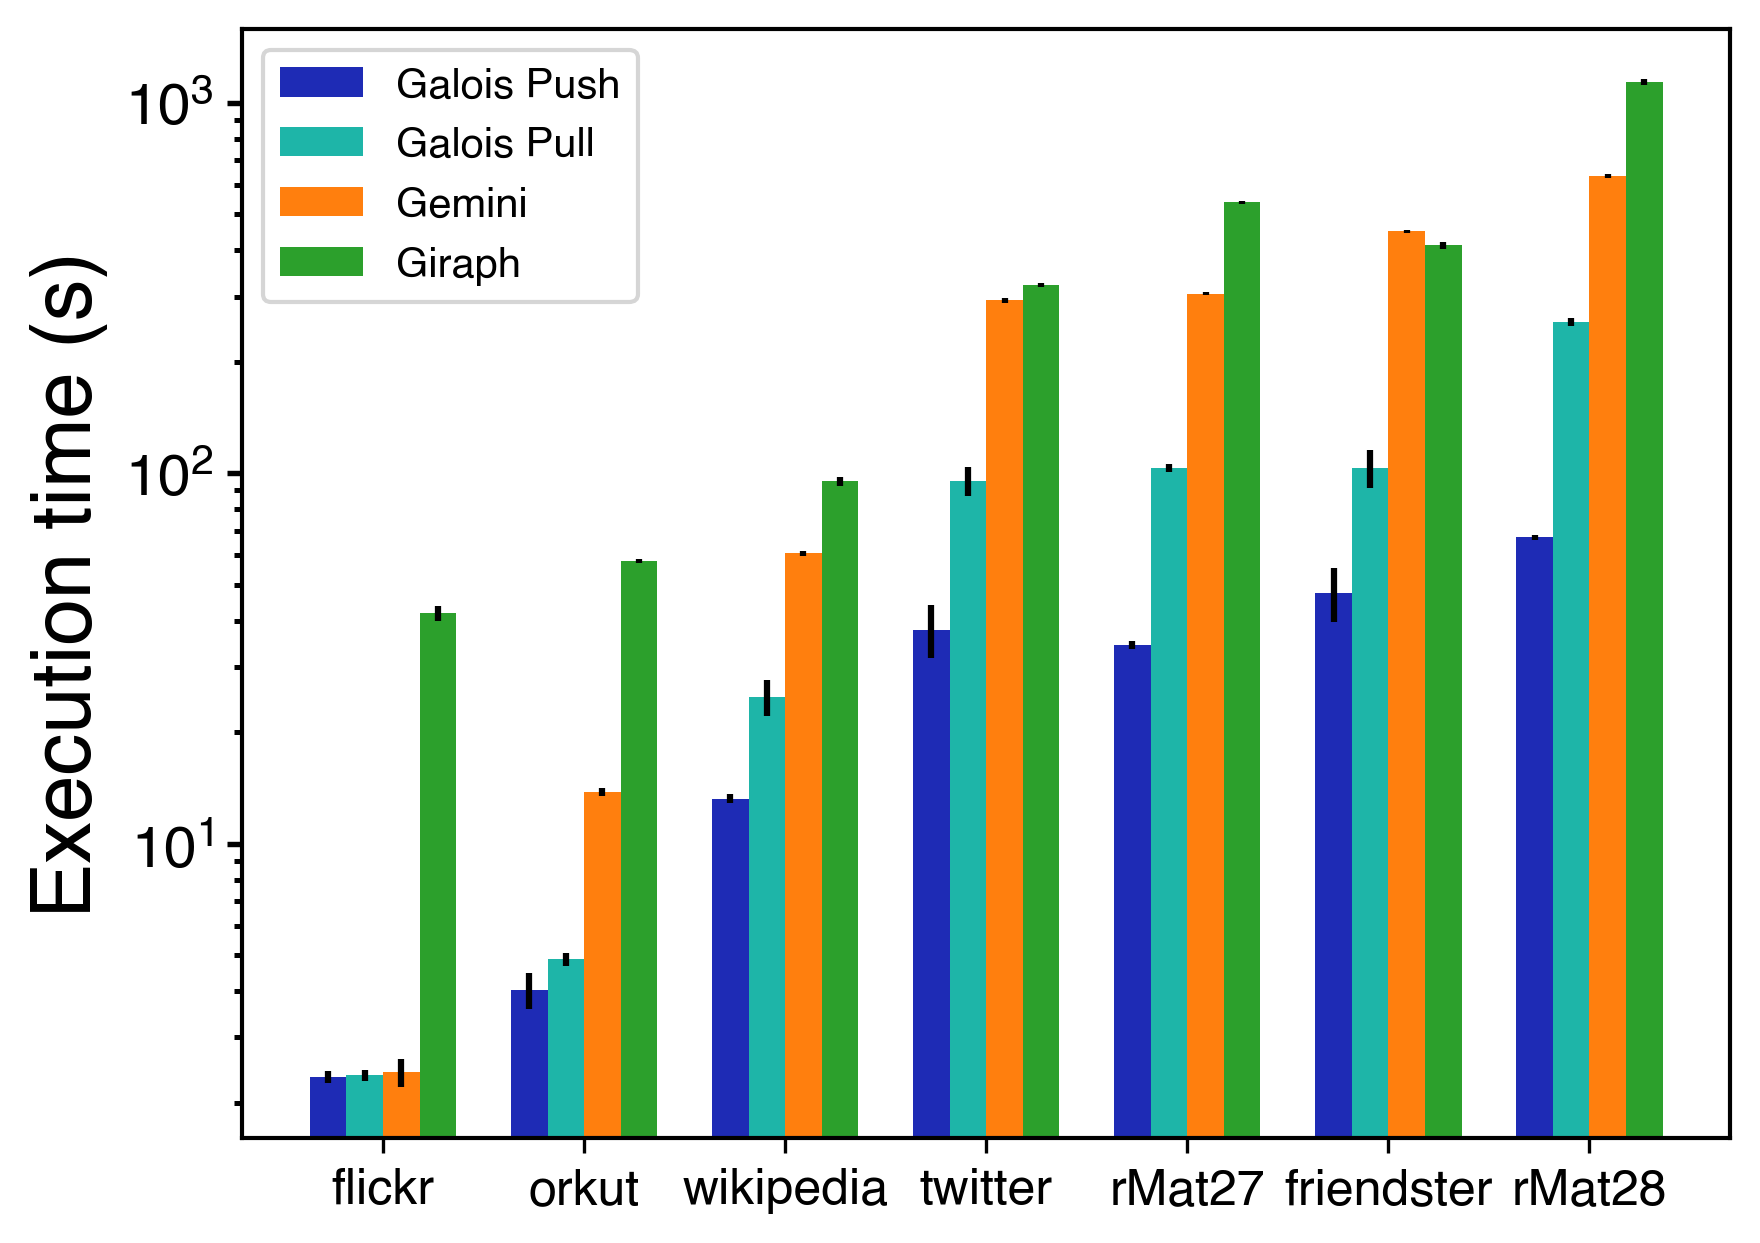
\includegraphics[width=\linewidth]{../../plots/distributedBFS_execTime.png}
		\caption{Execution times for distributed BFS}
		\label{fig:distributedBFS_exec}
	\end{subfigure}
	% \hfil
	% \begin{subfigure}{0.3\textwidth}
	% 	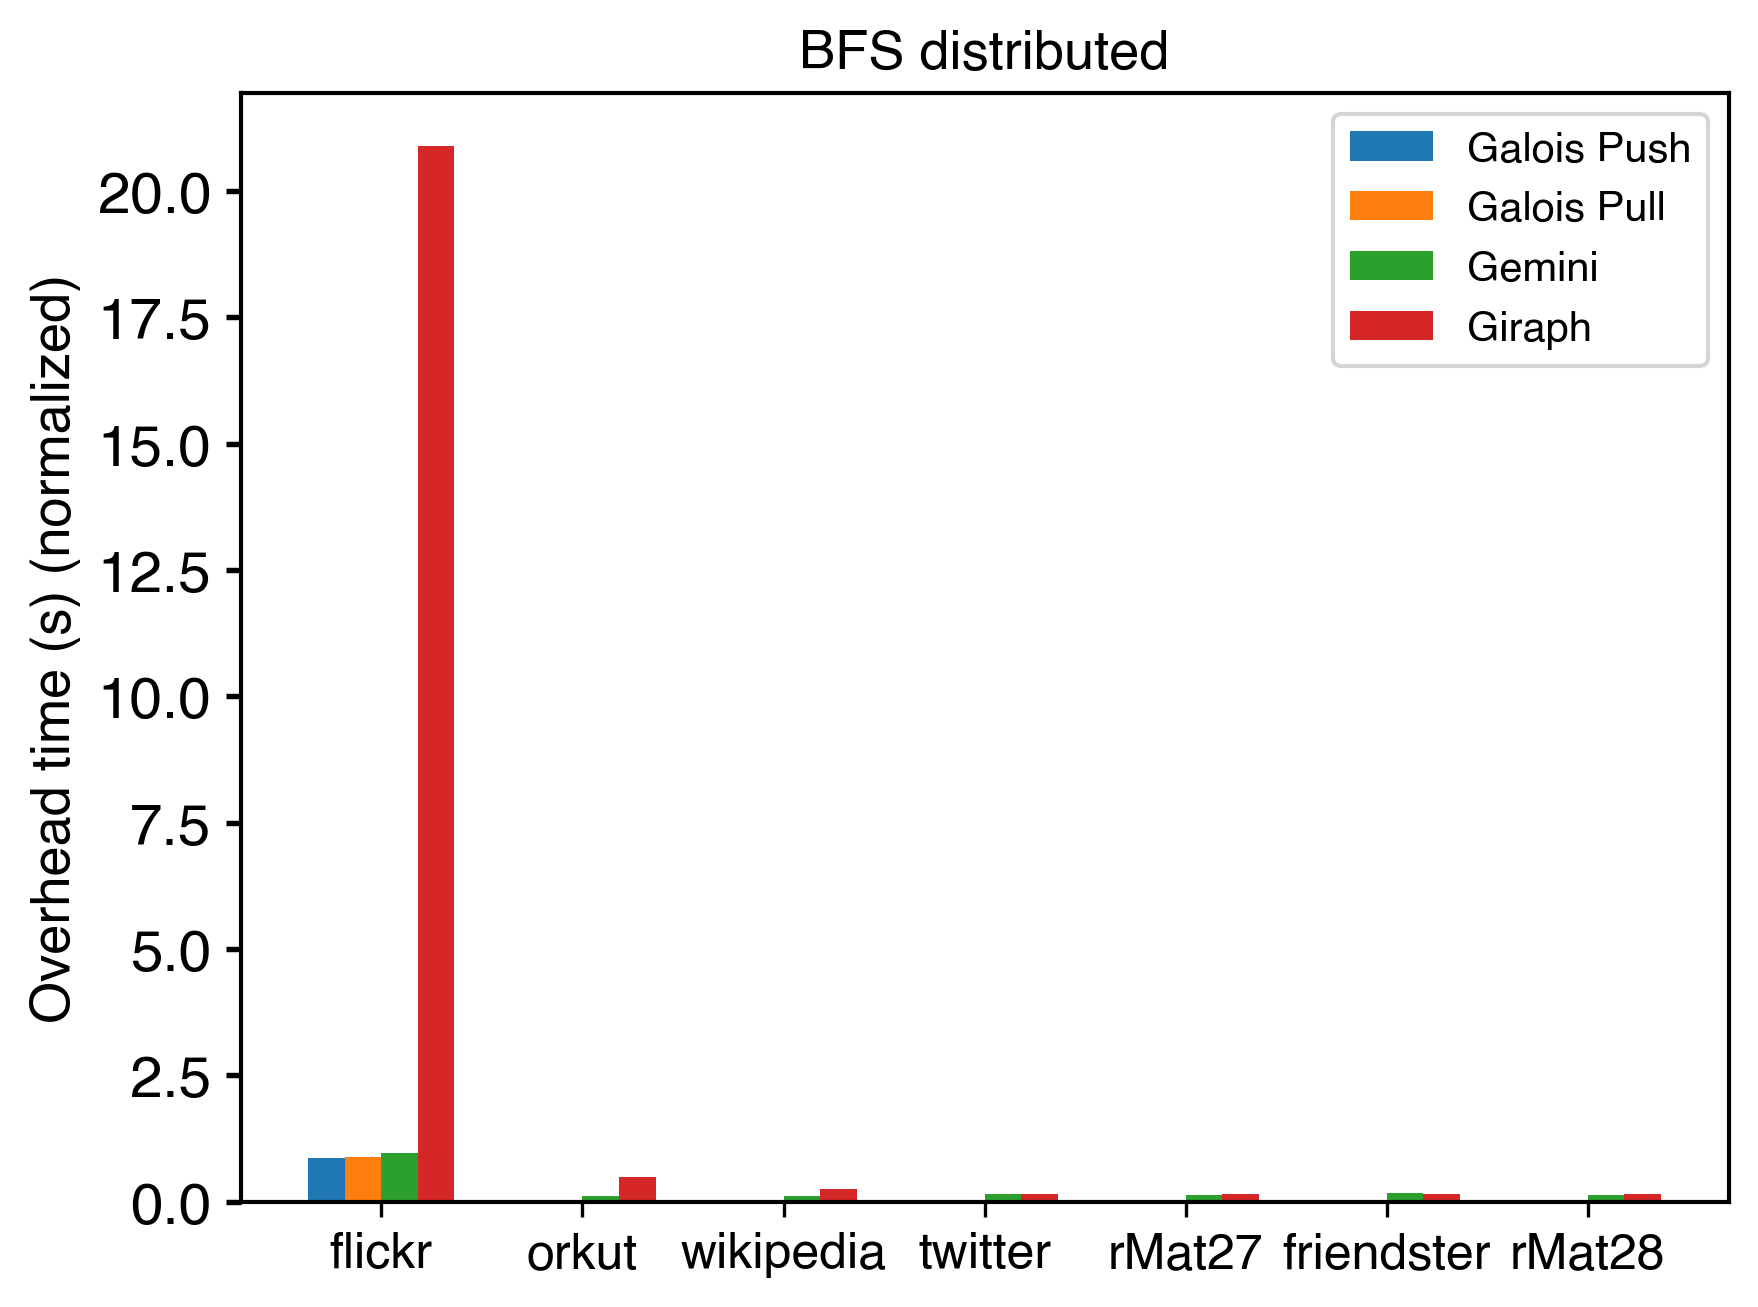
\includegraphics[width=\linewidth]{../../plots/distributedBFS_overheadTimeNormalized.png}
	% 	\caption{Overhead time normalized by the graph size in million edges}
	% 	\label{fig:distributedBFS_overheadNormalized}
	% \end{subfigure}
	\caption{Average times on the distributed cluster, black bars represent one standard deviation in our testing}
	\label{fig:distributedBFS}
\end{figure}
For both the calculation and the execution times, Breadth-First Search shows similar behaviour as the distributed SSSP test case. This is expected since both are graph traversal algorithms starting in one source vertex.
Hence, calculation complexity for each node and communication overhead is similar.
All measurements can be seen in \autoref{fig:distributedBFS}.

First, the calculation times in \autoref{fig:distributedBFS_calc}. It shows Giraph having the shortest calculation times on the real-world graphs, while Giraph's calculatin times on both rMat27 and rMat28 are the worst of all frameworks. 

Comparing the execution times in \autoref{fig:distributedBFS_exec} results in the same findings as with SSSP. 
While Gemini can compete with Galois on the small flickr graph, moving to larger data sets shows the worse performance of Gemini compared to Galois.

Much like when running SSSP, Giraph is slowest on all but one graph. Only on friendster is Gemini marginally slower, which was also the case for SSSP.

Both Galois implementations are again similar to the behaviour on SSSP.
Galois Push is generally faster than the Pull alternative while both Push and Pull versions are faster than Gemini and Giraph across all graphs.
This makes Galois Push the clear winner for distributed BFS.

